\documentclass[12pt, a4paper]{article}
\usepackage{caption}
\usepackage{graphicx}
\usepackage{hyperref}
\hypersetup{
    colorlinks,
    citecolor=black,
    filecolor=black,
    linkcolor=black,
    urlcolor=black
}
\usepackage{listings}
\usepackage{tikz-network}
\usepackage{amsmath, amsfonts, amssymb, amsthm}
\usepackage{algpseudocode}
\usepackage{algorithm}
\title{Algortihms and datastructures}
\date{2022}
\author{Kristoffer Klokker}
\begin{document}
	\maketitle
	\clearpage
	\tableofcontents
	\clearpage
		\section{Algorithm analyse}
			An algorithm must stop for all input and give the correct output.\\
			An algorithms quality is determined from:
			\begin{itemize}
				\item Speed
				\item Memory used
				\item Complexity of implmentation
				\item Other use cases like stability
			\end{itemize}
			\subsection{Algorithm speed}
				The measure speed and memory the worst case of the algorithm is always used due to its simplicity in calculations and gurantee. \\
				The measurement is used as a function of input size using the big O notation, which says for a given input with $n$ size it will take $n^2$  time to run for example.\\
				In reality the speed of an algorithm is not equivalent to the input size due to small constant in every operation but these are so miniscule, they should not be considered. A function may be tuned to have lower constants but this is more a topic for theoretical algorithm optimization.\\
				When comparing algorithm speed the math relations symbols are replaced as such:
				\begin{itemize}
					\item $= -\; \Theta$ Theta
					\item $\leq -\; O$ O
					\item $\geq - \;\Omega$ Omega
					\item $< -\; o$ little o
					\item $> - \;\omega$ little omega
				\end{itemize}
				When comparing the speed of two algorithms the following methods can be used:
				\begin{align*}
					\lim\limits_{n\rightarrow \infty}\frac{f(n)}{g(n)}>&0  &&f(n)=\Theta(g(n))\\
					\lim\limits_{n\rightarrow \infty}\frac{f(n)}{g(n)}=&0  &&f(n)=o(g(n))
				\end{align*}
				The generel speeds of alogirthms in order is:
				$$1,\; \log_2n,\; \sqrt{n},\; n,\; n\log_2n,\; n\sqrt{n},\; n^2,\; n^3,\; n^{10},\; 2^n$$
			\subsection{Ram-model}
				To analyze an algorithm a model is used most often the ram model.
				The ram model is a very simple interpretation of a computer.\\
				The model consist of a CPU, memory and basic operation (add, sub, mult, shift, move, jump)\\
				The time of the algorithm is then measured in amount of basic operations done.\\
				The memory is determined as the amount of memory cell used.
		\section{Sorting algorithms}
			Sorting algorithms are used to sort an array of items in an ascending order.\\
			\subsection{Insertionsort}
				One of the most simple sorting algorithms.\\
				Works by going through the list from index 1 and moves moves every entry before the element 1 up until the element is to the right of an element smaller than the element.\\
				This will therefore have a run time of $O(n^2)$ due to the scenario where the array is in decending order where it will moves $n-1,n-2,..,1$ elements which is $\sum\limits_{j=1}^nj=\frac{(n-1)n}{2}\leq\frac{n^2-n}{2}=n^2$
				\begin{algorithmic}[1]
					\State Insertion-Sort($A,n$)
					\For{$j=1$}{$n$}
						\State $key = A[j]$
						\State $i=j-1$
						\While {$i\geq0$ and $A[i] > key$}
							\State $a[i+1]=A[i]$
							\State $i = i-1$
						\EndWhile
						\State $A[i+1]=key$
					\EndFor
				\end{algorithmic}
			\subsection{Selectionsort}
				Selectionsort is done by taking all elements and then searching for the smallest element and inserting it into the list.\\
				This will result in the same run time $O(n^2)$ due to the same reasoning as insertionsort.\\
				\begin{algorithmic}[1]
					\State Selection-Sort($A,n$)
					\State Array output $= new Array(n)$
					\State $i = 0$
					\While {$i<n$}
						\State $output[i] = A[i]$
						\State $A[i].remove()$
						\State $i++$
					\EndWhile
				\end{algorithmic}
			\subsection{Merge sort}
				Merge sort is an sorting algorithm which is based on the simple merge of two sorted list. Here a new list is created and for every element of the two list, is the lowest value choosen from the first place of the list and putted into the new list. This is is done until both list are empty and when sorting the undefined element is simply equal to infinity when compared.\\[5mm]
				To make this into an sorting algorithm, every element in an unsorted list is made into to list of length 1. Then merge is performed on the lists in pairs of two, from which new sorted lists emerges. This is done until a single lists is left with all the elements which is now sorted. \\[4mm]
				 The speed of this sorting algorithm will therefore be $n\lceil\log_2n\rceil$ due to for every level of merge there will be performed $n$ operations. The amount of levels of merges are equal to $\log_2n$ due to first there will be $n$ lists, then $n/2$ lists, and then $n/2^2$. This will continue until $n/2^k=1$ which rearranged to find $k$ will be $log_2n=k$.\\
				 The ceiling of $\log_2n$ is due to in scenarios where the list length is not a potens of two and a list has no pair in this case it will go on to the next level and thus creating a new level once the list has 1 more item than a potens of two.
				 \begin{figure}
				 	\centering
				 	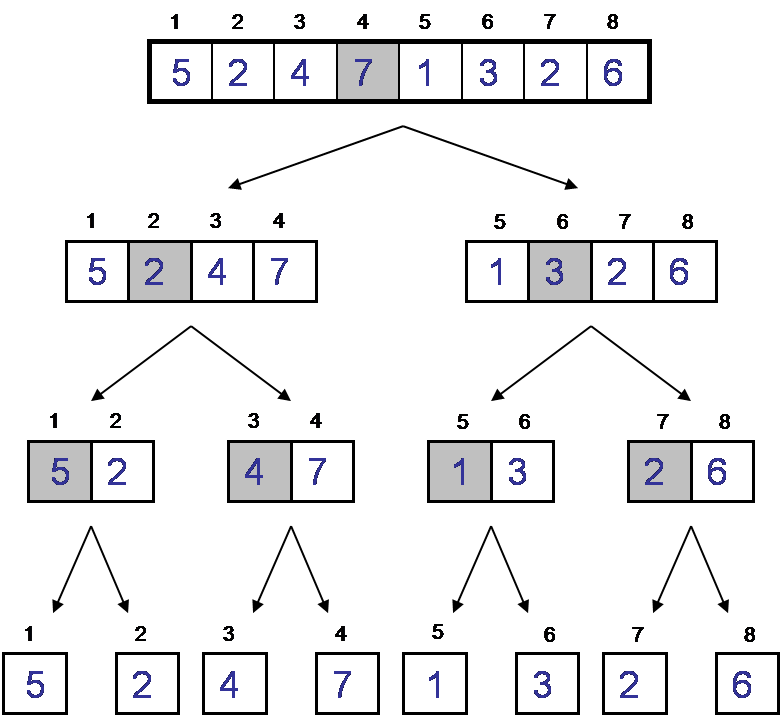
\includegraphics[width=300px]{assets/mergeSort.png}
				 	\caption{Merge sort list split up illustration from j2eereference.com}
				\end{figure}
			\subsection{Quick sort}
				A recursive sorting algorithm which runs mostly at $O(n\log n)$ time but worst case is $O(n^2)$.\\
				The sorting algorithm is smart due to it not needing subarrays copies and working in the original array.\\
				The main idea, is choosing an element in the array, then sorting everything in two baskets lower or equal and higher.\\
				Then the element is placed between the two baskets and quick sort is ran upon the two baskets.
				\begin{algorithmic}[1]
					\State Quick-Sort($A,p,r$)
					\If {$r \leq p$} \State return; \EndIf
					\State $i = p$
					\For {$j=p$ to $r$}
						\If {$A[j] \leq x$}
							\State $temp = A[i]$;
							\State $A[i] = A[j]$;
							\State $A[j] = temp$;
							\State $i=i+1$;
						\EndIf
					\EndFor
					\State $temp = A[i]$;
					\State $A[i] = A[r]$;
					\State $A[r] = temp$;
					\State $Quick-Sort(A,p,i-1)$;
					\State $Quick-Sort(A,i+1,r)$;
				\end{algorithmic}
				The arguments is the array $A$ the start of the sort $p$ and the end $r$.\\
				Here it is seen that in the for loop if the current element is smaller than the choosen element it is switched with the first element in larger basket such that the smaller basket is in front.\\
				In case the element is larger nothing is done. Then at the end the choosen element is switched with the first element of the larger bucket.
			\subsection{Heap sort}
				Heap sort is based on the Heap and runs in $O(n\log n)$ and uses no extra space. The heap which is a binary tree which follows heap order. The heap order dictates that a parent should always be greater or equal to its children. \\
				The tree should also have heap shape, which is all branches should be the saem height with a maximum difference of 1. In case of a larger branch it should be on the left side of the tree.\\
				This heap can is illustrated as a tree but is actually an array. Here the arrays first entry is the root, the roots children will then be at index 2 times index and 2 times index + 1\\
				This means the parent is at $\lfloor i/2 \rfloor$ relative to the child.
				\begin{figure}[h!]
					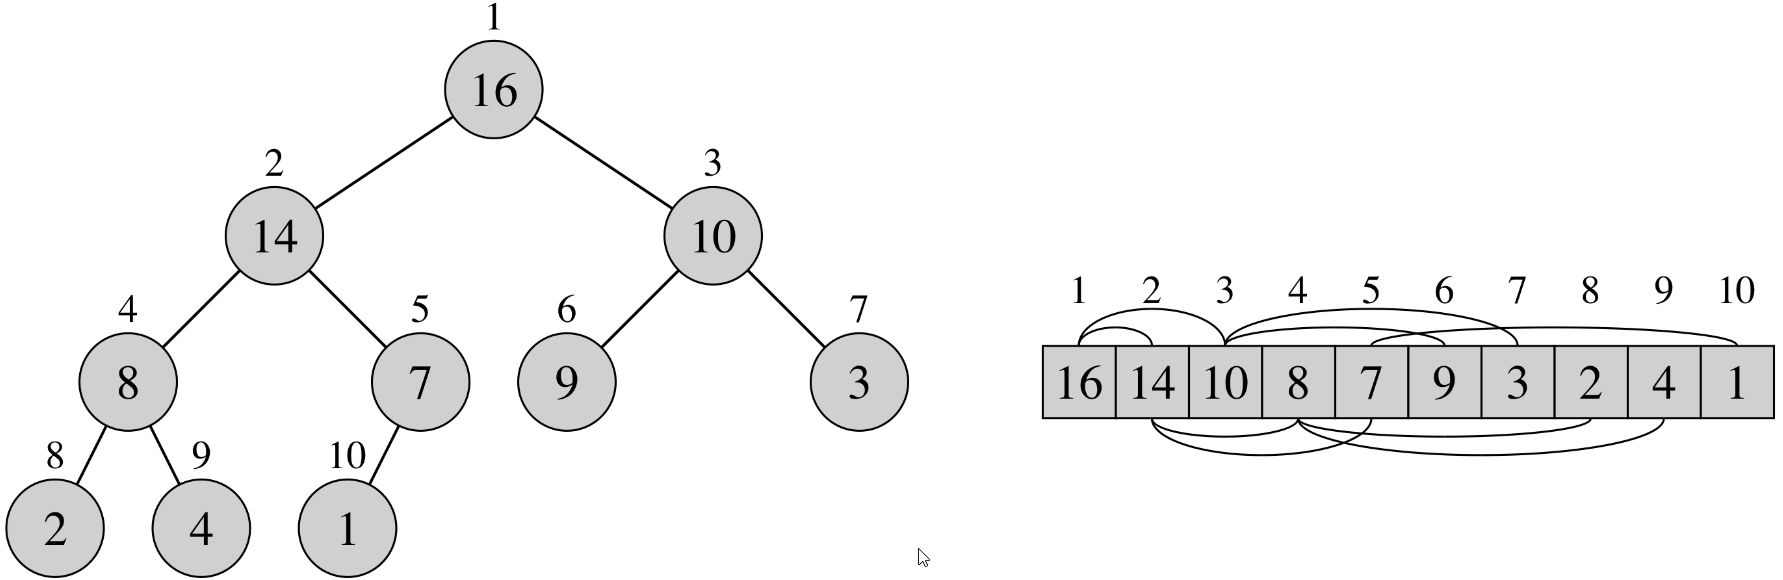
\includegraphics[width=300px]{assets/heapAsArray.png}
					\center
					\caption{The heap illustration and the heap array}
				\end{figure}
				Heap sort then uses the heap array, and when sorting the first entry or the root is switched with the last entry of the heap array.\\
				By this the size of the heap array shrinks with 1 and the rest of the array is the sorted array.\\
				When switched the heap is reconstructed.\\
				The reconstruction process is as follows:
				\begin{algorithmic}[1]
					\State Max-Heapify($A,i,n$)
					\State $l = 2i$;
					\State $r =2i+1$;
					\If {$l\leq n$ and $A[l] > A[i]$}
						\State $largest = l$;
					\Else
						\State $largest = i$;
					\EndIf
					\If {$r \leq n$ and $A[r] > A[largest]$}
						\State $largest = r$;
					\EndIf
					\If {$largest != i$}
						\State $temp = A[i]$;
						\State $A[i] = A[largest]$;
						\State $A[largest] = temp$;
						\State $Max-Heapify(A,largest,n)$;
					\EndIf
				\end{algorithmic}
				The $n$ is used as the length of the heap and $i$ is the current node to check.\\
				The first if check if the left child is larger, the second checks if the right child is larger, and the third check if something should be changed and if then call itself upon the newly changed child.\\
				With this function in mind heap sort becomes: 
				\begin{algorithmic}[1]
					\State HeapSort($A,n$)
						\State Max-Heapify(A,n);
						\For {$i=n$; $2 < i$; $i--$;}
							\State $temp = A[i]$;
							\State $A[i] = A[0]$;
							\State $A[0] = temp$;
							\State Max-Heapify($A,1,i-1$);
						\EndFor
				\end{algorithmic}
				The run time of this is $O(n\log n)$ dut to the trees height will maximally be $\log n$ which will be the number of exhanges $n$ times.
		\section{algorithms}
			\subsection{Maximum summation of sequential elements in array}
				The most simple version of this, is two pointers with start of seqence and end, where for each element in the array the start is appointed from which all possible ends if summed and the largest value is taken.\\
				This means the algorithm will take $O(n^3)$ due to first every element being appointed as start, from which all elements is tested as the end of sequence, from which the summation is done. This will round up to the worst case being $O(n^3)$\\
				This can be optimized to a run time of $O(n)$, by instead of recalculating everything for every pointer a pointer is started at the start from which an end pointer is also at the start.\\
				Here the largest summation is found, if it is larger than the best sequence it is assigned. Then the end pointer is moved forward and the new element is summed to the recent best sequence. If the sequence summation is now below zero the start pointer is moved to the end otherwise the end pointer is moved forward.
				\begin{algorithmic}[1]
					\State MaxSequence($A$)
					\State $max = 0$
					\State $tempMax = 0$
					\State $i = 0$
					\While {$i<A.length$}
						\State $tempMax = max(tempMax + A[i], 0)$
						\State $max = max(max, tempMax)$
						\State $i++$
					\EndWhile
				\end{algorithmic}
		\section{Divide-and-Conquer algorithms}
			The same as recursive algorithms.\\
			When illustrated a tree is often used to describe the calls and calls backs
				
	
				
\end{document}